\documentclass[conference]{IEEEtran}
\usepackage{amsmath,amssymb,amsthm}
\usepackage{graphicx}
\usepackage{booktabs}
\usepackage[hidelinks]{hyperref}
\usepackage{cite}
\newcommand{\accTdc}{33.3\%}
\newcommand{\accUci}{76.8\%}
\newcommand{\armAdaptTenMean}{6.3\%}
\newcommand{\armAdaptTenMoves}{74.9\%}
\newcommand{\armAdaptTenWorst}{8.8\%}
\newcommand{\armAfterTenMoves}{35.5\%}
\newcommand{\armBeforeTen}{17.8\%}
\newcommand{\armFixedMean}{20.5\%}
\newcommand{\fixedMeanTdc}{5.2\%}
\newcommand{\fixedMeanUci}{2.8\%}
\newcommand{\fixedWorstTdc}{26.5\%}
\newcommand{\fixedWorstUci}{24.9\%}
\newcommand{\gripGesture}{45\%}
\newcommand{\gripMisG}{4.3\%}
\newcommand{\gripMisM}{4.3\%}
\newcommand{\gripMotion}{69\%}
\newcommand{\keptConfPersTdc}{6}
\newcommand{\keptConfPersUci}{6}
\newcommand{\keptConfTdc}{6}
\newcommand{\keptConfUci}{6}
\newcommand{\keptNaiveTdc}{6}
\newcommand{\keptNaiveUci}{6}
\newcommand{\keptOwnTdc}{6}
\newcommand{\keptOwnUci}{6}
\newcommand{\keptVotePersTdc}{6}
\newcommand{\keptVotePersUci}{6}
\newcommand{\keptVoteTdc}{6}
\newcommand{\keptVoteUci}{6}
\newcommand{\nPeople}{91}
\newcommand{\nRuns}{1{,}365}
\newcommand{\nViol}{0}
\newcommand{\ownAccTdc}{85.6\%}
\newcommand{\ownAccUci}{93.6\%}
\newcommand{\ownFiveMovesUci}{88.3\%}
\newcommand{\pCalTdc}{<0.001}
\newcommand{\pCalUci}{0.008}
\newcommand{\pTwentyTwoOwn}{98.5\%}
\newcommand{\pTwentyTwoShared}{39.6\%}
\newcommand{\rfFixed}{0.6\%}
\newcommand{\rfKeptConf}{6}
\newcommand{\rfTunedFive}{16.7\%}
\newcommand{\rhoAccUci}{-0.60}
\newcommand{\rhoCalTdc}{0.73}
\newcommand{\rhoCalUci}{0.43}
\newcommand{\sharedFiveMovesUci}{40.5\%}
\newcommand{\shiftAcc}{47.2\%}
\newcommand{\shiftAdaptCI}{4.9--5.0\%}
\newcommand{\shiftAdaptMean}{4.9\%}
\newcommand{\shiftAdaptMoves}{31.5\%}
\newcommand{\shiftAdaptWorst}{5.0\%}
\newcommand{\shiftAfterMoves}{0.0\%}
\newcommand{\shiftBeforeKept}{1}
\newcommand{\shiftBeforeMean}{12.0\%}
\newcommand{\shiftBeforeWorst}{37.0\%}
\newcommand{\shiftFixedMean}{46.1\%}
\newcommand{\shiftFixedWorst}{82.1\%}
\newcommand{\shiftOracleMoves}{14.0\%}
\newcommand{\shiftSparseKept}{0}
\newcommand{\sparseKeptlimbpos}{6}
\newcommand{\sparseKepttdc}{6}
\newcommand{\sparseKeptuci}{6}
\newcommand{\tunedFiveTdc}{10.4\%}
\newcommand{\tunedFiveUci}{6.3\%}
\newcommand{\tunedKeptTdc}{0}
\newcommand{\tunedKeptUci}{0}
\newcommand{\wilcoxOracleP}{10^{-6}}
\newcommand{\wilcoxP}{10^{-15}}
\newcommand{\worstConfPersUci}{9.2\%}
\newcommand{\worstConfUci}{23.1\%}
\newcommand{\examplePerson}{8}

\newtheorem{proposition}{Proposition}
\newcommand{\target}{\alpha}

\begin{document}

\title{Misfire-Rate Guarantees for Myoelectric Control Under Distribution Shift: Adaptive Rejection on Top of Recalibration}

\author{\IEEEauthorblockN{Kishore Nuthalapati}
\IEEEauthorblockA{Independent researcher, Alpharetta, GA, USA\\
kishorenuthalapat@gmail.com}}

\maketitle

\begin{abstract}
Pattern-recognition myoelectric controllers act only when classifier confidence exceeds a fixed threshold, which leaves the rate of unintended movements uncontrolled for new users and after recording conditions change. We set the threshold from a target misfire rate instead. A conformal threshold calibrated across previous users bounds a new user's expected misfire rate. An adaptive threshold updated from feedback bounds each user's own misfire rate on any sequence of decisions, and an importance-weighted variant keeps the bound, in expectation, when feedback arrives on only a random subset of decisions. In leave-one-person-out evaluation on four public datasets (\nPeople{} people), a $45^\circ$ armband rotation made LibEMG's default threshold move the device unintentionally on \shiftFixedMean{} of decisions. No threshold alone restored control: the adaptive threshold met a 5\% target but performed only \shiftAdaptiveMoves{} of intended movements. Retraining the classifier from the same feedback restored accuracy to \shiftRetrainAcc{} but left \shiftRetrainFixedOver{} of \shiftN{} users above 5\% with the default threshold. Combining retraining with the adaptive threshold kept every one of the \nPeople{} users at or below the target at all six levels tested on all four datasets, at a cost of \deltaMovesRAvsRF{} percentage points of correct movements relative to retraining alone. Code is public and plugs into LibEMG.
\end{abstract}

\section{Introduction}

Myoelectric prostheses classify surface electromyography (EMG) into motions and update the device every few tens of milliseconds. A wrong decision moves the device when the user did not ask for it, for example opening the hand while it holds a cup. Confidence-based rejection, in which the controller holds still unless the classifier's top probability exceeds a threshold, reduces such errors and improves usability~\cite{scheme2013,robertson2019}.

The threshold is normally a fixed number; LibEMG, a widely used open-source library for myoelectric control, defaults to 0.90~\cite{eddy2023}. The error rate that number produces depends on the classifier, the user and the recording conditions. EMG patterns differ between people~\cite{yang2024} and shift with electrode displacement and arm position~\cite{campbell2024,fougner2011}, and class probabilities are often overconfident on the data a model was fit to.

We ask whether a threshold can be set from a target such as ``move unintentionally on at most 5\% of decisions'' and whether that target holds for people the model has never seen and after conditions change. Our contributions are:
\begin{enumerate}
\item A \emph{conformal threshold} for an unchanged rejection controller, using conformal risk control~\cite{angelopoulos2024} with people as the exchangeable unit, with an exact extension to majority voting.
\item An \emph{adaptive threshold} with a deterministic per-user bound under any decision sequence, and a label-efficient, importance-weighted variant whose bound holds in expectation over all decisions when only a random share of them receive feedback.
\item Evidence on four public datasets that a threshold alone cannot restore control after a large change, that retraining restores accuracy but not the target, and that the two together keep every user at the target with little loss of movement.
\end{enumerate}

\section{Related Work}

Scheme \emph{et al.} introduced confidence-based rejection with class-specific thresholds~\cite{scheme2013}. Menon \emph{et al.} chose class-specific thresholds automatically from ROC curves on training data~\cite{menon2015}, and Robertson \emph{et al.} found in real-time use that usability peaks at intermediate thresholds that depend on the classifier~\cite{robertson2019} and separated errors caused by the classifier from those caused by the user~\cite{robertson2018}. Other work improves the confidence score itself~\cite{tam2024,aydogan2026}; any such score can be used with our thresholds. Context-informed incremental learning adapts the classifier from task context and improves resilience to electrode shift~\cite{campbell2024}; we use the same kind of feedback to retrain and show that a threshold on top is still needed for a per-user guarantee. Conformal prediction gives finite-sample guarantees for any model~\cite{vovk2005}; conformal risk control extends them to monotone losses~\cite{angelopoulos2024}, and adaptive conformal inference maintains long-run guarantees under shift~\cite{gibbs2021,angelopoulos2023pid}. We are not aware of their application to rejection thresholds in myoelectric control.

\section{Methods}

\subsection{Decisions, misfires and missed movements}
For decision $i$ the classifier outputs a class $\hat y_i$ with confidence $c_i$, its top probability. The rejection controller outputs $\hat y_i$ if $c_i>t$ and ``hold still'' otherwise. One class is \emph{rest}, which also holds the device still. A \emph{misfire} is a decision on which the device moves in a way the user did not intend: the output is a motion class other than rest and differs from the intended class $y_i$. This covers false activations during rest and wrong motions. A confident rest prediction while the user wants to move is a \emph{missed movement}, which costs usability but does not move the device. Person $p$'s misfire rate over their decisions $W_p$ is
\begin{equation}
R_p(t) = \frac{1}{|W_p|}\sum_{i\in W_p} \mathbf{1}\left[c_i > t,\ \hat y_i \ne y_i,\ \hat y_i \ne \text{rest}\right],
\end{equation}
which is non-increasing in $t$. We also report \emph{correct movements}: the share of decisions with an intended motion on which the controller performs that motion.

\subsection{Conformal threshold across people}
Decisions within a person are strongly dependent, so we treat people as exchangeable. For a held-out user, the other $n$ people are split into five folds and each is scored by a model trained on the other four, so every calibration person is scored by a model that never saw them. With $\bar R(t)$ the mean of their misfire curves,
\begin{equation}
\hat t = \inf\left\{t : \tfrac{n}{n+1}\bar R(t) + \tfrac{1}{n+1} \le \target\right\}.
\end{equation}
If the new person is exchangeable with the calibration people, $\mathbb{E}[R_{n+1}(\hat t)] \le \target$~\cite{angelopoulos2024}. Targets below $1/(n+1)$ cannot be met. A \emph{personal check} computes the smallest threshold meeting $\target$ on the user's own calibration recording and uses the larger of the two; since $R_p$ is non-increasing, this preserves the guarantee. For LibEMG's majority vote, each voted curve is replaced by its running maximum from the right and computed exactly at every threshold by evaluating the vote in the $k+1$ intervals between the $k$ confidences in each window; the implementation matches LibEMG's output decision for decision.

\subsection{Adaptive threshold with a per-user guarantee}
When conditions change after calibration we use feedback. With $s_i=\min(-\log_{10}(1-c_i),S)$, $S=6$, the controller acts if $s_i>\tau_i$, and after decision $i$
\begin{equation}
\tau_{i+1} = \max\left(\tau_i + \eta\,(m_i - \target),\ 0\right),
\end{equation}
where $m_i$ indicates a misfire and $\eta=0.5$.

\begin{proposition}
If $\tau_1 \le S$, then for every $T$ and every sequence of decisions,
$\frac{1}{T}\sum_{i=1}^{T} m_i \le \target + \frac{S+\eta-\tau_1}{\eta T}.$
\end{proposition}
\begin{proof}
$\tau$ rises only after a misfire, which requires $s_i>\tau_i$ and hence $\tau_i<S$, so $\tau_{i+1}<S+\eta$; when $\tau_i\ge S$ the controller cannot act and $\tau$ falls. Thus $\tau_i\le S+\eta$ throughout. Summing the update, $\eta\sum_i(m_i-\target)=\tau_{T+1}-\tau_1-c$ with $c\ge0$ the total added by the floor at zero.
\end{proof}

\emph{Sparse feedback.} If only a random share $p$ of decisions receive feedback, updating on those alone makes $\tau$ move $p$ times slower. Instead we update on every decision with an importance-weighted misfire:
\begin{equation}
\tau_{i+1} = \max\left(\tau_i + \eta\,(F_i m_i/p - \target),\ 0\right),
\end{equation}
where $F_i=1$ if decision $i$ receives feedback, drawn independently with probability $p$.

\begin{proposition}
If $\tau_1\le S$, then for every $T$ and every decision sequence in which decision $i$ may depend on $F_1,\dots,F_{i-1}$ but not on $F_i,F_{i+1},\dots$ (for example, a model retrained on the labels received so far), $\frac{1}{T}\sum_i F_i m_i/p \le \target + \frac{S+\eta/p-\tau_1}{\eta T}$ surely, and $\mathbb{E}\big[\frac{1}{T}\sum_i m_i\big]$ obeys the same bound.
\end{proposition}
\begin{proof}
The argument of Proposition~1 with jump $\eta/p$ gives the first claim. Since $m_i$ is determined by $F_1,\dots,F_{i-1}$ and $F_i$ is drawn independently of them, $\mathbb{E}[F_i m_i]=p\,\mathbb{E}[m_i]$; take expectations.
\end{proof}

\subsection{Retraining with an adaptive threshold}
The same feedback can be used to retrain the classifier. Every 100 decisions (5\,s), the model is refit on its training data plus every post-change decision whose label is known so far, and each block is scored by a model that has not seen it. The adaptive threshold then runs on this stream unchanged, so Propositions~1 and~2 still apply. Retraining needs the intended class, which a cued task provides; the adaptive threshold alone needs only whether a movement was wrong.

\section{Experimental Setup}

\begin{table}[t]
\caption{Datasets. ``Change'' separates calibration from testing.}
\label{tab:data}
\centering
\footnotesize
\begin{tabular}{@{}lrrl@{}}
\toprule
Dataset & People & Classes & Change \\
\midrule
UCI EMG for Gestures~\cite{krilova2018} & 36 & 6 & Later session \\
3DC~\cite{coteallard2019} & 22 & 11 & Later session \\
CIIL electrode shift~\cite{campbell2024} & 21 & 5 & $45^\circ$ rotation \\
Limb position~\cite{fougner2011} & 12 & 8 & 4 new arm positions \\
\bottomrule
\end{tabular}
\end{table}

Table~\ref{tab:data} lists the datasets; each includes a rest class. EMG is cut into 250\,ms windows with a 50\,ms step, described by LibEMG's Hudgins time-domain features and classified by LibEMG's linear discriminant analysis (LDA), with a random forest as a robustness check.

\emph{Shared models (UCI, 3DC).} For each person, a model is trained on all other people, thresholds are chosen, and the person's later session is scored. Personal checks use only the person's first session.

\emph{User-specific models under change (all four datasets).} Each person's model is trained on the first half of their pre-change recordings; the second half is their calibration recording, and all post-change decisions in recording order form the test stream. Baselines are LibEMG's 0.90, per-class ROC thresholds on the user's calibration recording (Youden's index, after~\cite{menon2015}), conformal thresholds calibrated on other people before the change or after the same change (which requires such recordings to exist), and the best fixed threshold for each user chosen in hindsight. Feedback is given on every decision or on a random 10\%.

Targets are $\target\in\{3,5,7.5,10,15,20\}\%$. We report mean and worst-user misfire rates, users above target, and correct movements; a target is \emph{met on average} when the mean is at or below it.

\section{Results}

\subsection{New users with shared models}

\begin{table}[t]
\caption{Shared LDA models, unseen users: mean and worst misfire rate (\%), users above target, and correct movements (\%).}
\label{tab:shared}
\centering
\footnotesize
\setlength{\tabcolsep}{3pt}
\begin{tabular}{@{}llrrrrr@{}}
\toprule
Data & Cutoff & $\alpha$ & Mean & Worst & Over & Moves \\
\midrule
UCI & Fixed 0.90 (LibEMG) & -- & 2.8\% & 24.9\% & -- & 49.3\% \\
UCI & Tuned on training data & 5\% & 6.3\% & 32.7\% & 15/36 & 64.1\% \\
UCI & Conformal & 5\% & 2.1\% & 23.1\% & 4/36 & 42.3\% \\
UCI & Conformal + personal & 5\% & 1.5\% & 9.2\% & 4/36 & 40.5\% \\
UCI & Tuned on training data & 10\% & 12.9\% & 45.9\% & 19/36 & 81.5\% \\
UCI & Conformal & 10\% & 6.7\% & 32.7\% & 9/36 & 65.4\% \\
UCI & Conformal + personal & 10\% & 5.3\% & 14.9\% & 9/36 & 62.2\% \\
\midrule
3DC & Fixed 0.90 (LibEMG) & -- & 5.2\% & 26.5\% & -- & 14.8\% \\
3DC & Tuned on training data & 5\% & 10.4\% & 54.5\% & 11/22 & 23.7\% \\
3DC & Conformal & 5\% & 0.5\% & 5.2\% & 1/22 & 2.1\% \\
3DC & Conformal + personal & 5\% & 0.5\% & 5.2\% & 1/22 & 2.1\% \\
3DC & Tuned on training data & 10\% & 18.3\% & 76.6\% & 16/22 & 35.7\% \\
3DC & Conformal & 10\% & 5.3\% & 26.9\% & 4/22 & 15.0\% \\
3DC & Conformal + personal & 10\% & 3.4\% & 10.6\% & 1/22 & 12.6\% \\
\bottomrule
\end{tabular}

\end{table}

Without rejection, shared models reached \accUci{} (UCI) and \accTdc{} (3DC) accuracy on unseen users. Thresholds tuned on training data met \tunedKeptUci{} of 6 targets on UCI and \tunedKeptTdc{} on 3DC: at 5\%, new users saw \tunedFiveUci{} and \tunedFiveTdc{} (Table~\ref{tab:shared}). Conformal thresholds met all 6 targets on average on both datasets, with and without five-decision majority voting, and the personal check cut the worst UCI user at 5\% from \worstConfUci{} to \worstConfPersUci{}. With a random forest the tuned threshold met \rfKeptTuned{} of 6 targets (\rfTunedFive{} at 5\%), because the forest is nearly certain on its training data, while conformal thresholds met all \rfKeptConf{}. The average guarantee came at a high price on 3DC, where the shared model is weak: conformal thresholds performed \confFiveMovesTdc{} of intended movements at 5\%, against \ownMovesTdc{} for user-specific models without rejection.

\subsection{When conditions change}

\begin{table*}[t]
\caption{User-specific LDA models after a change, 5\% target (fixed and ROC thresholds have no target). Mean and worst-user misfire rate and correct movements (\%). Number of people in parentheses.}
\label{tab:drift}
\centering
\footnotesize
\setlength{\tabcolsep}{4.2pt}
\begin{tabular}{@{}lrrrrrrrrrrrr@{}}
\toprule
 & \multicolumn{3}{c}{Electrode shift (21)} & \multicolumn{3}{c}{Arm position (12)} & \multicolumn{3}{c}{UCI, later session (36)} & \multicolumn{3}{c}{3DC, later session (22)} \\
\cmidrule(lr){2-4}\cmidrule(lr){5-7}\cmidrule(lr){8-10}\cmidrule(lr){11-13}
Cutoff & Mean & Worst & Corr. & Mean & Worst & Corr. & Mean & Worst & Corr. & Mean & Worst & Corr. \\
\midrule
Fixed 0.90 (LibEMG) & 44.0 & 78.5 & 33 & 18.8 & 31.4 & 74 & 8.6 & 25.4 & 86 & 10.2 & 24.0 & 72 \\
ROC per class & 39.5 & 71.5 & 30 & 16.6 & 32.2 & 71 & 6.1 & 21.1 & 82 & 7.1 & 19.9 & 67 \\
Conformal, before change & 15.4 & 41.6 & 10 & 0.0 & 0.0 & 0 & 0.2 & 5.8 & 2 & 0.8 & 4.3 & 29 \\
Conformal, after change & 0.0 & 0.0 & 0 & 0.0 & 0.0 & 0 & 0.0 & 0.0 & 0 & 0.5 & 3.4 & 22 \\
Best fixed, hindsight & 3.5 & 5.0 & 8 & 4.9 & 5.0 & 55 & 3.1 & 5.0 & 64 & 5.0 & 5.0 & 63 \\
Adaptive & 4.9 & 5.0 & 19 & 3.9 & 5.0 & 68 & 3.4 & 5.2 & 78 & 3.7 & 4.7 & 69 \\
\midrule
Retrain + fixed 0.90 & 6.6 & 10.3 & 82 & 3.0 & 6.2 & 88 & 6.1 & 19.0 & 88 & 5.0 & 10.6 & 75 \\
Retrain + conformal & 1.5 & 6.2 & 20 & 0.0 & 0.0 & 0 & 0.1 & 2.1 & 1 & 0.3 & 1.6 & 24 \\
Retrain + adaptive & 2.0 & 3.9 & 80 & 1.6 & 2.8 & 89 & 2.2 & 4.6 & 81 & 3.0 & 3.8 & 77 \\
\midrule
10\% labels: adaptive (plain) & 5.2 & 8.3 & 10 & 4.5 & 5.3 & 59 & 3.1 & 8.3 & 65 & 3.4 & 4.8 & 56 \\
10\% labels: adaptive (weighted) & 5.0 & 7.4 & 10 & 3.9 & 5.4 & 55 & 3.4 & 10.0 & 62 & 3.8 & 6.2 & 60 \\
10\% labels: retrain + fixed & 13.0 & 25.3 & 70 & 6.2 & 13.3 & 84 & 7.7 & 23.6 & 87 & 7.5 & 18.4 & 74 \\
10\% labels: retrain + adaptive & 3.3 & 5.7 & 52 & 2.4 & 3.8 & 77 & 2.6 & 10.0 & 66 & 3.4 & 4.5 & 63 \\
\bottomrule
\end{tabular}

\end{table*}

\begin{figure*}[t]
\centering
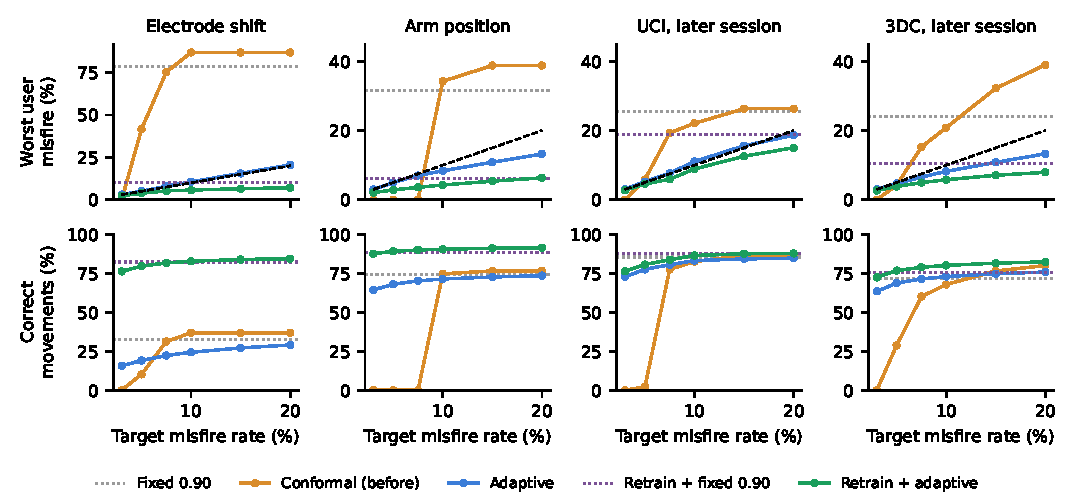
\includegraphics[width=\textwidth]{figures/drift.pdf}
\caption{User-specific models after a change. Top: worst user's misfire rate against the target (dashed: target). Bottom: correct movements. Dotted lines: LibEMG's 0.90 without and with retraining. Only retraining plus the adaptive threshold keeps the worst user at the target while moving nearly as often as retraining alone.}
\label{fig:drift}
\end{figure*}

\emph{A threshold alone.} After the $45^\circ$ rotation, user-specific models fell to \shiftAcc{} accuracy and the default threshold misfired on \shiftFixedMean{} of decisions (worst user \shiftFixedWorst{}; Table~\ref{tab:drift}). Per-class ROC thresholds gave \shiftRocPerClassMean{}. A conformal threshold calibrated before the rotation met \shiftConformalBeforeKept{} of 6 targets on average (\shiftConformalBeforeMean{} at 5\%, worst \shiftConformalBeforeWorst{}); calibrated on other people after the rotation, it met every target by never moving. The adaptive threshold held the worst user at \shiftAdaptiveWorst{} but performed only \shiftAdaptiveMoves{} of intended movements, because with \shiftAcc{} accuracy few confident decisions are right. On the milder changes the adaptive threshold alone worked well (Fig.~\ref{fig:drift}), and across all \nPeople{} users it performed more correct movements than the best fixed threshold chosen in hindsight (Wilcoxon signed-rank, $p<\wilAvsOracle$).

\emph{Retraining alone.} Retraining every 5\,s raised post-rotation accuracy to \shiftRetrainAcc{}, but with the default threshold the mean misfire rate was \shiftRetrainFixedMean{} and \shiftRetrainFixedOver{} of \shiftN{} users exceeded 5\%. Across all four datasets, \poolRFOver{} of \nPeople{} users exceeded 5\% (worst \poolRFWorst{}).

\emph{Retraining with the adaptive threshold.} With both, no user exceeded the target at any of the six levels on any dataset. At 5\%, the mean misfire rate was \shiftRetrainAdaptiveMean{} after the rotation (95\% bootstrap interval over users \shiftRetrainAdaptiveCI{}, worst \shiftRetrainAdaptiveWorst{}) with \shiftRetrainAdaptiveMoves{} correct movements, against \shiftRetrainFixedMoves{} for retraining with the default threshold. Pooled over datasets, correct movements were \poolRAMoves{} against \poolRFMoves{}, and misfires were lower ($p<\wilRAvsRF$). Proposition~1 was violated in \nViol{} of \nRuns{} runs, as it must be; we report this only as a check of the implementation.

\begin{figure}[t]
\centering
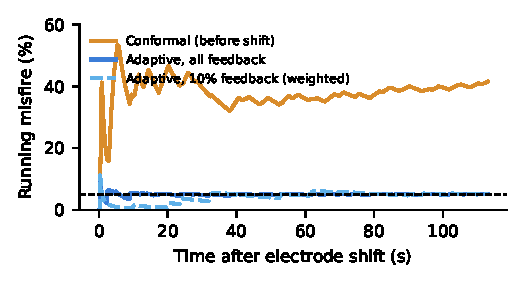
\includegraphics[width=\columnwidth]{figures/one_user.pdf}
\caption{Running misfire rate of electrode-shift participant \examplePerson{}, the worst user under the conformal threshold calibrated before the shift, at a 5\% target (dashed), with a threshold alone (no retraining).}
\label{fig:oneuser}
\end{figure}

\subsection{Feedback on 10\% of decisions}
Updating only on labeled decisions met the 5\% target on average for arm position, UCI and 3DC but met \shiftAdaptivetenpctKept{} of 6 targets after the rotation. The importance-weighted update met \shiftAdaptivetenpctIpwKept{} of 6 there, and its weighted bound held in all \nRunsIpw{} runs, but the expectation guarantee does not bound each user: \shiftAdaptivetenpctIpwOver{} of \shiftN{} exceeded 5\% (worst \shiftAdaptivetenpctIpwWorst{}). With retraining from the same 10\% of labels plus the adaptive threshold, the mean met every target on every dataset, \poolRAtenOver{} of \nPeople{} users exceeded 5\% (worst \poolRAtenWorst{}), and correct movements were \poolRAtenMoves{}, against \poolRFtenOver{} users above 5\% for retraining with the default threshold.

\subsection{Acting on motions, and who goes over}
Three 3DC classes close the hand (power, chuck and pinch grip). Summing their probabilities and rejecting on motions, calibrated identically, let user-specific models perform the grip motion on \gripMotion{} of grip decisions instead of \gripGesture{} at a 7.5\% target with an unchanged misfire rate (\gripMisM{}). With shared models, the calibration-recording misfire rate predicted the test misfire rate ($\rho=\rhoCalUci$, UCI; $\rho=\rhoCalTdc$, 3DC; both $p<0.001$), an early warning for users who need retraining.

\section{Discussion}

A threshold chosen from a target makes behavior predictable in units that matter to users and clinicians, but it cannot create correct decisions that the classifier does not make. After a large change, a threshold alone can only trade unintended movements for missed ones; retraining restores accuracy but not a bound. Used together, retraining supplies accuracy and the adaptive threshold supplies the bound, and because the threshold relaxes as the retrained model improves, the bound costs little movement. The conformal threshold remains useful when previous users were recorded under the conditions of use and no feedback is available.

\emph{Limitations.} All results are offline: recorded EMG replayed through the controller, without a user adapting in closed loop and without a physical device, and offline error is known to be an imperfect proxy for real-time usability~\cite{robertson2019}. Participants were able-bodied, and calibration and test were recorded on the same day. Feedback assumes a cued task; in daily use it would have to come from implicit signals such as the user undoing a movement. With 10\% feedback, the guarantee is in expectation and some users exceed the target. Conformal thresholds need many calibration people (targets below $1/(n+1)$ are unreachable) and were conservative. Every misfire counts equally, although opening during a grasp is worse than a wrong wrist rotation; a weighted loss fits the same framework.

\section{Conclusion}

On \nPeople{} people across four datasets, choosing rejection thresholds from a target misfire rate turned a confidence number into a guarantee. Conformal thresholds met targets on average for new users; adaptive thresholds held each user at the target under any change; and only retraining combined with an adaptive threshold kept every user at the target while performing nearly as many intended movements as retraining alone. Future work is real-time evaluation with amputee participants, multi-day data and implicit feedback. Code: \url{https://github.com/kishoren18-hue/steadyhand}.

\section*{Acknowledgment}
Claude (Anthropic), an AI system, was used to write the experiment and analysis code, to generate the figures and tables from the results, and to draft the text of all sections. The author designed the study, directed every revision, checked the results and proofs, and takes full responsibility for the content. We thank the authors of LibEMG and of the four datasets for making them public.

\begin{thebibliography}{99}
\footnotesize
\bibitem{scheme2013} E.~Scheme, B.~Hudgins, and K.~Englehart, ``Confidence-based rejection for improved pattern recognition myoelectric control,'' \emph{IEEE Trans. Biomed. Eng.}, vol.~60, no.~6, 2013.
\bibitem{robertson2019} J.~W. Robertson, K.~B. Englehart, and E.~J. Scheme, ``Effects of confidence-based rejection on usability and error in pattern recognition-based myoelectric control,'' \emph{IEEE J. Biomed. Health Inform.}, vol.~23, no.~5, pp.~2002--2008, 2019.
\bibitem{robertson2018} J.~W. Robertson, K.~B. Englehart, and E.~J. Scheme, ``Rejection of systemic and operator errors in a real-time myoelectric control task,'' in \emph{Proc. IEEE EMBC}, 2018, pp.~5640--5643.
\bibitem{menon2015} R.~Menon, G.~Di~Caterina, H.~Lakany, L.~Petropoulakis, B.~A. Conway, and J.~J. Soraghan, ``Automatic misclassification rejection for LDA classifier using ROC curves,'' in \emph{Proc. IEEE EMBC}, 2015, pp.~482--485.
\bibitem{eddy2023} E.~Eddy, E.~Campbell, A.~Phinyomark, S.~Bateman, and E.~Scheme, ``LibEMG: An open source library to facilitate the exploration of myoelectric control,'' \emph{IEEE Access}, vol.~11, 2023.
\bibitem{yang2024} J.~Yang, M.~Soh, V.~Lieu, D.~J. Weber, and Z.~Erickson, ``EMGBench: Benchmarking out-of-distribution generalization and adaptation for electromyography,'' in \emph{Adv. Neural Inf. Process. Syst.}, 2024.
\bibitem{campbell2024} E.~Campbell, E.~Eddy, S.~Bateman, U.~C\^ot\'e-Allard, and E.~Scheme, ``Context-informed incremental learning improves both the performance and resilience of myoelectric control,'' \emph{J. NeuroEng. Rehabil.}, vol.~21, 2024.
\bibitem{fougner2011} A.~Fougner, E.~Scheme, A.~D.~C. Chan, K.~Englehart, and \O.~Stavdahl, ``Resolving the limb position effect in myoelectric pattern recognition,'' \emph{IEEE Trans. Neural Syst. Rehabil. Eng.}, vol.~19, no.~6, 2011.
\bibitem{angelopoulos2024} A.~N. Angelopoulos, S.~Bates, A.~Fisch, L.~Lei, and T.~Schuster, ``Conformal risk control,'' in \emph{Proc. Int. Conf. Learn. Represent.}, 2024.
\bibitem{gibbs2021} I.~Gibbs and E.~Cand\`es, ``Adaptive conformal inference under distribution shift,'' in \emph{Adv. Neural Inf. Process. Syst.}, 2021.
\bibitem{angelopoulos2023pid} A.~N. Angelopoulos, E.~J. Cand\`es, and R.~J. Tibshirani, ``Conformal PID control for time series prediction,'' in \emph{Adv. Neural Inf. Process. Syst.}, 2023.
\bibitem{tam2024} S.~Tam \emph{et al.}, ``Towards robust and interpretable EMG-based hand gesture recognition using deep metric meta learning,'' arXiv:2404.15360, 2024.
\bibitem{aydogan2026} Y.~Ayd\u{o}\u{g}an and \.{I}.~Cant\"urk, ``Uncertainty-aware single-channel surface EMG classification for low-resource hand gesture recognition: A subject-independent evaluation,'' \emph{Med. Biol. Eng. Comput.}, 2026.
\bibitem{vovk2005} V.~Vovk, A.~Gammerman, and G.~Shafer, \emph{Algorithmic Learning in a Random World}. New York: Springer, 2005.
\bibitem{krilova2018} N.~Krilova, I.~Kastalskiy, V.~Kazantsev, V.~Makarov, and S.~Lobov, ``EMG data for gestures,'' UCI Machine Learning Repository, 2018.
\bibitem{coteallard2019} U.~C\^ot\'e-Allard \emph{et al.}, ``Deep learning for electromyographic hand gesture signal classification using transfer learning,'' \emph{IEEE Trans. Neural Syst. Rehabil. Eng.}, vol.~27, no.~4, 2019.
\end{thebibliography}

\end{document}
